Assim como os outros métodos de Newton, esse método tem como intenção facilitar o cálculo da Hessiana. Deseja-se chegar a ela sem derivar duas vezes a função objetivo. As iterações são regidas por:
\begin{equation}
x^{k+1}=x^k + \alpha_kd^k = x^k - \alpha[F^k]^{-1}g^k
\end{equation}
onde $F^k$ contem informações sobre a Hessiana $G^k$ e deve ser obtido de forma simples. A tarefa de obter $F^k$ é substituída pela de obter sua inversa $H^k = [F^k]^{-1}$. Em cada passo esta matriz deve exibir, de algum modo, características da Hessiana, ou melhor, de sua inversa. Vejamos como conseguir isso. Utilizando a expansão em série de Taylor do gradiente de f, podemos notar que H, em cada iteração, pode ser delimitado pela relação
\begin{equation}
	H^{k+1} \gamma^{k} = \delta^{k} = \left\{
	\begin{tabular}{c}
	\gamma^{k} = g^{k+1} - g^{k}\\ 
	\delta^{k} = x^{k+1} - x^{k} 
	\end{tabular}
	\end{equation}
chamada de condição de quase-Newton. Para gerar matrizes H satisfazendo esta restrição utilizamos, em nosso programa, a fórmula de Broyden-Fletcher-Goldfarb-Shanno (BFGS):
\begin{equation}
H^{k+1} = H - \frac{\delta \gamma^T H + H \gamma \delta^T}{\delta^T \gamma} + \Bigg( 1 + \frac{\gamma^T H \gamma}{\delta^T \gamma}\Bigg) \frac{\delta \delta^T}{\delta^T \gamma}
\end{equation}

Para comprovar a eficiência do método, o testamos utilizando as seguintes funções:
\begin{itemize}
	\item $ f_1(x,y) = x^2 + y^2$
	\item $ f_2(x,y) = -e^{-x^2 -y^2}$
	\item $ f_3(x,y) = cos(\frac{xy}{5})+sin(\frac{xy}{5}) $
	\item $ f_4(x,y) = |x+y| $
\end{itemize}

Os resultados foram os seguintes:
\begin{figure}[H]
	\begin{center}	
		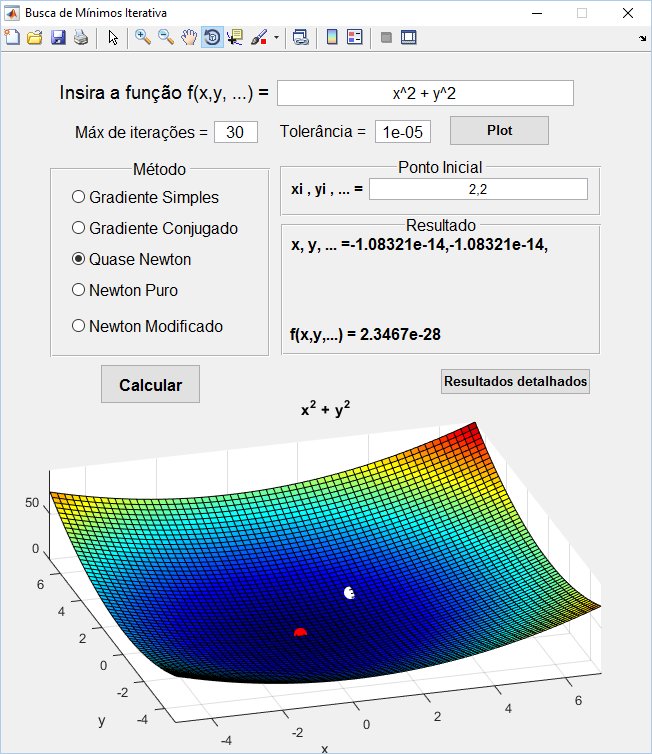
\includegraphics[width=12cm]{../quase_newton/f1_gui.PNG}
		\caption{Janela de inicialização de $ f_1(x,y) $}
		\label{fig:f1_gui_qn}
	\end{center}
\end{figure}



\begin{figure}[H]
	\begin{center}	
		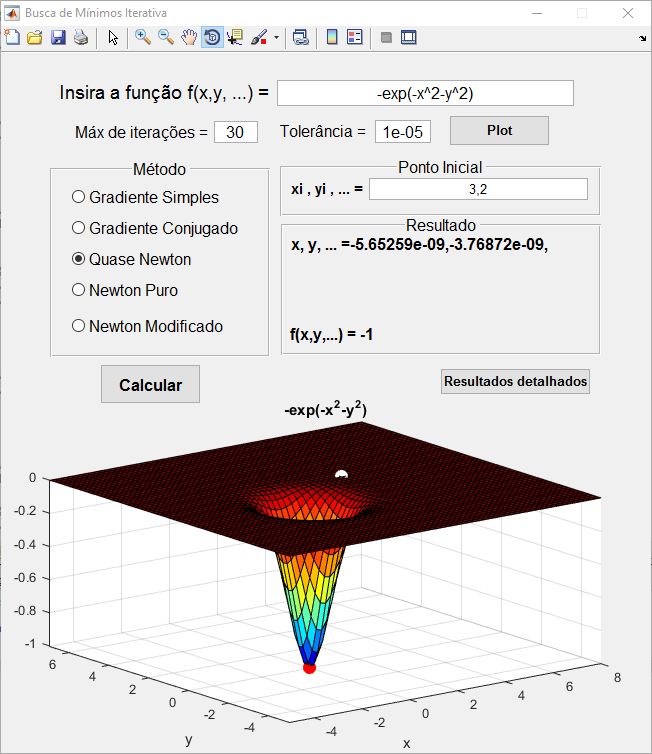
\includegraphics[width=12cm]{../quase_newton/f2_gui.PNG}
		\caption{Janela de inicialização de $ f_2(x,y) $}
		\label{fig:f2_gui_qn}
	\end{center}
\end{figure}



\begin{figure}[H]
	\begin{center}	
		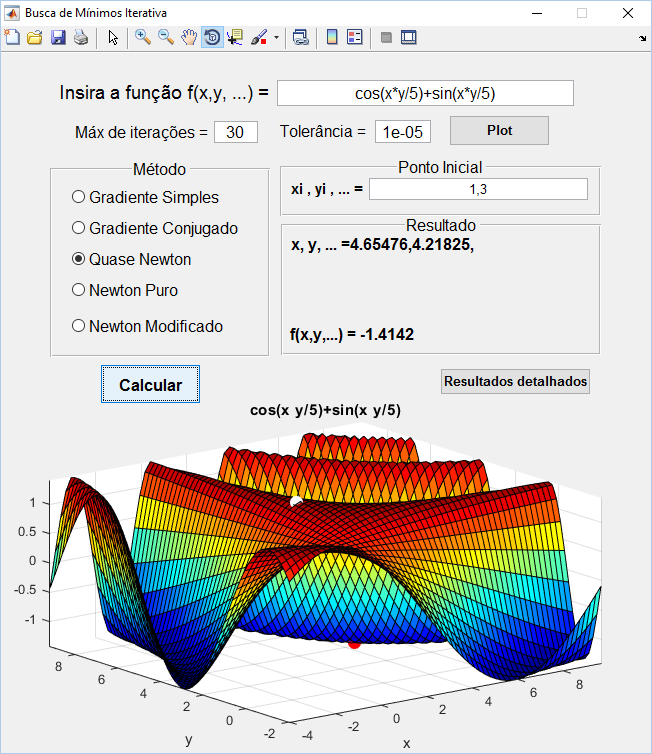
\includegraphics[width=12cm]{../quase_newton/f3_gui.PNG}
		\caption{Janela de inicialização de $ f_3(x,y) $}
		\label{fig:f3_gui_qn}
	\end{center}
\end{figure}



\begin{figure}[H]
	\begin{center}	
		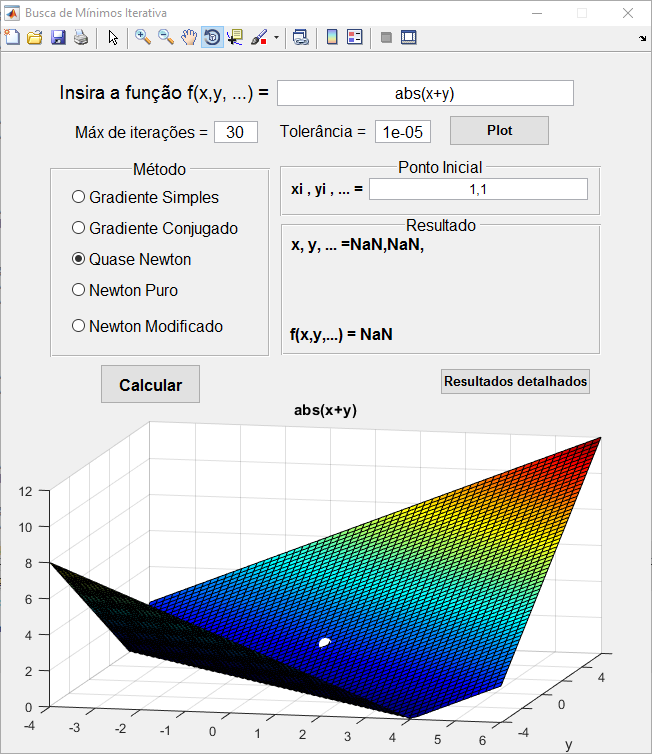
\includegraphics[width=12cm]{../quase_newton/f4_gui.PNG}
		\caption{Janela de inicialização de $ f_4(x,y) $}
		\label{fig:f4_gui_qn}
	\end{center}
\end{figure}

\newpage